\documentclass[11pt, a4paper]{article}

% Fonts and Encoding
\usepackage[utf8]{inputenc}
\usepackage[T1]{fontenc}
\usepackage{lmodern}

% Math and Symbols
\usepackage{amsmath, amssymb, amsthm, amsfonts, mathrsfs, mathtools}

% Layout and Geometry
\usepackage{geometry}
\geometry{a4paper, margin=1in}

% Formatting and Graphics
\usepackage{graphicx, xcolor, enumitem, booktabs, array, tabularx}

% TikZ for Illustrations
\usepackage{tikz}
\usetikzlibrary{arrows.meta, positioning, shapes.geometric, calc, backgrounds, matrix}

% Clickable Links and TOC
\usepackage{hyperref}
\hypersetup{
    colorlinks=true,
    linkcolor=blue,
    filecolor=magenta,      
    urlcolor=cyan,
    pdftitle={Advanced Mathematics Topic: Functions},
}

% Theorem Environments
\newtheorem{theorem}{Theorem}[section]
\newtheorem{lemma}[theorem]{Lemma}
\newtheorem{proposition}[theorem]{Proposition}
\newtheorem{corollary}[theorem]{Corollary}
\theoremstyle{definition}
\newtheorem{definition}{Definition}[section]
\newtheorem{axiom}{Axiom}[section]
\newtheorem{example}{Example}[section]
\theoremstyle{remark}
\newtheorem{remark}{Remark}[section]

% Custom Commands (Enforced standard notation)
\newcommand{\R}{\mathbb{R}}
\newcommand{\N}{\mathbb{N}}
\newcommand{\Z}{\mathbb{Z}}
\newcommand{\Q}{\mathbb{Q}}
\newcommand{\E}{\mathbb{E}}
\newcommand{\Prob}{\mathbb{P}}
\newcommand{\F}{\mathcal{F}}

\begin{document}

\title{\textbf{Advanced Abstract Mathematics: Functions and Mappings}}
\author{Tashfeen Omran}
\date{\today}
\maketitle

\tableofcontents
\newpage

\section{Part 1: Comprehensive Introduction, Context, and Prerequisites}

\subsection{Core Concepts \& Axioms}
In the rigorous study of abstract mathematics, the concept of a \textbf{function} is formalized through the lens of set theory. Before defining a function, we must understand a \textbf{relation}. Let $A$ and $B$ be nonempty sets. A relation $R$ from $A$ to $B$ is defined as a subset of the Cartesian product $A \times B$. 

A \textbf{function} $f$ from $A$ to $B$, denoted as $f: A \to B$, is a specific type of relation with a strict constraint: every element $a \in A$ must be the first coordinate of \textit{exactly one} ordered pair in $f$. 
\begin{itemize}
    \item \textbf{Domain:} The set $A$ is called the domain of $f$, denoted $\text{dom}(f)$.
    \item \textbf{Codomain:} The set $B$ is called the codomain of $f$.
    \item \textbf{Image:} If $(a, b) \in f$, we write $b = f(a)$. The element $b$ is the image of $a$ under $f$.
    \item \textbf{Range:} The set of all actual outputs, $\text{range}(f) = \{f(x) : x \in A\}$, is a subset of the codomain $B$.
    \item \textbf{Preimage (Inverse Image):} For a subset $D \subseteq B$, the preimage is $f^{-1}(D) = \{a \in A : f(a) \in D\}$.
\end{itemize}

\subsection{Intuition and Set-Theoretic Foundations}
Intuitively, a function is a deterministic machine or a "mapping." If you feed it an input from set $A$, it will reliably produce exactly one output in set $B$. In set-theoretic terms, a function partitions its domain based on the elements of the codomain they map to. The strict requirement that an input cannot map to multiple outputs ensures logical consistency, which is paramount when functions are used to define random variables in probability spaces or transformations in linear algebra.

\subsection{Historical Context and Motivation}
The modern definition of a function evolved over centuries. In the 18th century, mathematicians like Johann Bernoulli and Leonhard Euler viewed functions strictly as analytic expressions or formulas (e.g., $f(x) = x^2$). However, as mathematics expanded into Fourier series and real analysis, this definition proved too restrictive. In the 19th century, Peter Dirichlet and Richard Dedekind generalized the concept, defining a function purely as an arbitrary correspondence between sets, independent of any algebraic formula. This paradigm shift was necessary to resolve foundational crises in analysis and paved the way for modern topology and measure theory.

\subsection{Key Theorems, Lemmas, and Formulas}
\begin{theorem}[Equality of Functions]
Two functions $f: A \to B$ and $g: A \to B$ are equal, written $f = g$, if and only if $f(a) = g(a)$ for all $a \in A$.
\end{theorem}

\begin{theorem}[Cardinality of Function Spaces]
Let $A$ and $B$ be finite sets. The set of all functions from $A$ to $B$ is denoted by $B^A$. The number of such functions is given by $|B^A| = |B|^{|A|}$.
\end{theorem}

\subsection{Prerequisites}
To master this chapter, the reader must be proficient in:
\begin{itemize}
    \item \textbf{Set Theory:} Union, intersection, set difference, and Cartesian products.
    \item \textbf{Logic:} Universal ($\forall$) and existential ($\exists$) quantifiers, and contrapositive statements.
    \item \textbf{Basic Algebra:} Solving inequalities and understanding absolute values.
\end{itemize}

\newpage
\section{Part 2: Detailed Homework Solutions}

\subsection{Problem 10.1}
\textbf{Problem:} Let $A = \{a, b, c, d\}$ and $B = \{x, y, z\}$. Then $f = \{(a, y), (b, z), (c, y), (d, z)\}$ is a function from $A$ to $B$. Determine $\text{dom}(f)$ and $\text{range}(f)$.

\textbf{Solution:}
By definition, the domain of a function $f$ given as a set of ordered pairs is the set of all first coordinates.
\[ \text{dom}(f) = \{a, b, c, d\} = A \]
The range of $f$ is the set of all second coordinates that appear in the ordered pairs.
\[ \text{range}(f) = \{y, z\} \]
$\blacksquare$

\subsection{Problem 10.2}
\textbf{Problem:} Let $A = \{1, 2, 3\}$ and $B = \{a, b, c, d\}$. Give an example of a relation $R$ from $A$ to $B$ containing exactly three elements such that $R$ is not a function from $A$ to $B$. Explain why $R$ is not a function.

\textbf{Solution:}
Let $R = \{(1, a), (1, b), (2, c)\}$. 
This relation $R$ contains exactly three elements. It is not a function from $A$ to $B$ for two distinct reasons:
1. The element $1 \in A$ is the first coordinate of two distinct ordered pairs, $(1, a)$ and $(1, b)$, violating the rule that each input must map to exactly one output.
2. The element $3 \in A$ is not the first coordinate of any ordered pair in $R$, violating the rule that every element in the domain must be mapped to some element in the codomain.
$\blacksquare$

\subsection{Problem 10.3}
\textbf{Problem:} Let $A$ be a nonempty set. If $R$ is a relation from $A$ to $A$ that is both an equivalence relation and a function, then what familiar function is $R$? Justify your answer.

\textbf{Solution:}
\textbf{Proof Technique: Direct Deduction.}
Since $R$ is an equivalence relation on $A$, it must be reflexive. By the definition of reflexivity, for every $x \in A$, the ordered pair $(x, x) \in R$.
Since $R$ is also a function from $A$ to $A$, every element $x \in A$ must be the first coordinate of \textit{exactly one} ordered pair in $R$. 
Because we already established that $(x, x) \in R$ for all $x \in A$, there can be no other ordered pairs $(x, y)$ in $R$ where $x \neq y$. 
Therefore, $R = \{(x, x) : x \in A\}$. This is the definition of the \textbf{identity function} on $A$, commonly denoted as $i_A(x) = x$.
$\blacksquare$

\subsection{Problem 10.4}
\textbf{Problem:} For the given subset $A_i$ of $\R$ and the relation $R_i$ ($1 \le i \le 3$) from $A_i$ to $\R$, determine whether $R_i$ is a function from $A_i$ to $\R$.

\textbf{Solution:}
\textbf{(a)} $A_1 = \R, R_1 = \{(x, y) : x \in A_1, y = 4x - 3\}$
For every $x \in \R$, the expression $4x - 3$ evaluates to a single, unique real number $y$. Thus, every $x \in A_1$ is related to exactly one $y \in \R$. \textbf{Yes, $R_1$ is a function.}

\textbf{(b)} $A_2 = [0, \infty), R_2 = \{(x, y) : x \in A_2, (y + 2)^2 = x\}$
Let $x = 1 \in A_2$. We solve for $y$:
\[ (y + 2)^2 = 1 \implies y + 2 = 1 \quad \text{or} \quad y + 2 = -1 \implies y = -1 \quad \text{or} \quad y = -3 \]
Since both $-1 \in \R$ and $-3 \in \R$, the element $x = 1$ is related to two distinct elements in the codomain. \textbf{No, $R_2$ is not a function.}

\textbf{(c)} $A_3 = \R, R_3 = \{(x, y) : x \in A_3, (x + y)^2 = 4\}$
Let $x = 0 \in A_3$. We solve for $y$:
\[ (0 + y)^2 = 4 \implies y^2 = 4 \implies y = 2 \quad \text{or} \quad y = -2 \]
The element $x = 0$ is related to two distinct elements. \textbf{No, $R_3$ is not a function.}
$\blacksquare$

\subsection{Problem 10.5}
\textbf{Problem:} Let $A$ and $B$ be nonempty sets and let $R$ be a nonempty relation from $A$ to $B$. Show that there exists a subset $A'$ of $A$ and a subset $f$ of $R$ such that $f$ is a function from $A'$ to $B$.

\textbf{Solution:}
\textbf{Proof Technique: Constructive Proof.}
Since $R$ is a nonempty relation from $A$ to $B$, there exists at least one ordered pair in $R$. Let $(a, b)$ be one such ordered pair, where $a \in A$ and $b \in B$.
Define the subset $A' \subseteq A$ as $A' = \{a\}$.
Define the subset $f \subseteq R$ as $f = \{(a, b)\}$.
We must verify that $f$ is a function from $A'$ to $B$. The domain of $f$ is the set of all first coordinates, which is exactly $\{a\} = A'$. For the single element $a \in A'$, there is exactly one ordered pair in $f$ starting with $a$, namely $(a, b)$. Thus, $a$ maps to exactly one element in $B$. Therefore, $f$ is a valid function from $A'$ to $B$.
$\blacksquare$

\subsection{Problem 10.6}
\textbf{Problem:} In each of the following, a function $f_i : A_i \to \R$ ($1 \le i \le 5$) is defined, where the domain $A_i$ consists of all possible real numbers $x$ for which $f_i(x)$ is defined. In each case, determine the domain $A_i$ and the range of $f_i$.

\textbf{Solution:}
\textbf{(a)} $f_1(x) = 1 + x^2$
Domain $A_1$: The expression $1 + x^2$ is defined for all real numbers. $A_1 = \R$.
Range: Since $x^2 \ge 0$ for all $x \in \R$, we have $1 + x^2 \ge 1$. The range is $[1, \infty)$.

\textbf{(b)} $f_2(x) = 1 - \frac{1}{x}$
Domain $A_2$: The expression is undefined when the denominator is zero. $A_2 = \R \setminus \{0\}$.
Range: Let $y = 1 - \frac{1}{x}$. Solving for $x$ yields $\frac{1}{x} = 1 - y \implies x = \frac{1}{1 - y}$. For $x$ to exist as a real number, we must have $1 - y \neq 0 \implies y \neq 1$. Thus, the range is $\R \setminus \{1\}$.

\textbf{(c)} $f_3(x) = \sqrt{3x - 1}$
Domain $A_3$: The argument of the square root must be non-negative. $3x - 1 \ge 0 \implies x \ge \frac{1}{3}$. $A_3 = [\frac{1}{3}, \infty)$.
Range: The principal square root function outputs all non-negative real numbers. Range is $[0, \infty)$.

\textbf{(d)} $f_4(x) = x^3 - 8$
Domain $A_4$: Polynomials are defined everywhere. $A_4 = \R$.
Range: The cubic function is continuous and unbounded in both directions. Range is $\R$.

\textbf{(e)} $f_5(x) = \frac{x}{x-3}$
Domain $A_5$: The denominator cannot be zero. $A_5 = \R \setminus \{3\}$.
Range: Let $y = \frac{x}{x-3}$. Solving for $x$:
\[ y(x-3) = x \implies xy - 3y = x \implies x(y-1) = 3y \implies x = \frac{3y}{y-1} \]
For $x$ to be a real number, $y \neq 1$. Furthermore, we must ensure $x \neq 3$. If $x = 3$, then $3 = \frac{3y}{y-1} \implies 3y - 3 = 3y \implies -3 = 0$, which is a contradiction. Thus $x$ is never $3$. The range is $\R \setminus \{1\}$.
$\blacksquare$

\subsection{Problem 10.7}
\textbf{Problem:} Let $A = \{3, 17, 29, 45\}$ and $B = \{4, 6, 22, 60\}$. A relation $R$ from $A$ to $B$ is defined by $a R b$ if $a + b$ is a prime. Is $R$ a function from $A$ to $B$?

\textbf{Solution:}
We must check if every element in $A$ relates to exactly one element in $B$.
\begin{itemize}
    \item For $a = 3$: $3+4=7$ (prime), $3+6=9$ (not), $3+22=25$ (not), $3+60=63$ (not). $3$ relates only to $4$.
    \item For $a = 17$: $17+4=21$ (not), $17+6=23$ (prime), $17+22=39$ (not), $17+60=77$ (not). $17$ relates only to $6$.
    \item For $a = 29$: $29+4=33$ (not), $29+6=35$ (not), $29+22=51 = 3 \times 17$ (not), $29+60=89$ (prime). $29$ relates only to $60$.
    \item For $a = 45$: $45+4=49$ (not), $45+6=51$ (not), $45+22=67$ (prime), $45+60=105$ (not). $45$ relates only to $22$.
\end{itemize}
Since every element in $A$ is related to exactly one element in $B$, \textbf{Yes, $R$ is a function.}
$\blacksquare$

\subsection{Problem 10.8}
\textbf{Problem:} Let $A = \{5, 6\}$, $B = \{5, 7, 8\}$ and $S = \{n : n \ge 3 \text{ is an odd integer}\}$. A relation $R$ from $A \times B$ to $S$ is defined as $(a, b) R s$ if $s \mid (a + b)$. Is $R$ a function from $A \times B$ to $S$?

\textbf{Solution:}
The domain is $A \times B = \{(5,5), (5,7), (5,8), (6,5), (6,7), (6,8)\}$. We must find all odd divisors $s \ge 3$ for the sum $a+b$ of each pair.
\begin{itemize}
    \item $(5,5) \implies a+b = 10$. Divisors of 10 are $1, 2, 5, 10$. The only odd divisor $\ge 3$ is $5$. $(5,5) R 5$.
    \item $(5,7) \implies a+b = 12$. Divisors of 12 are $1, 2, 3, 4, 6, 12$. The only odd divisor $\ge 3$ is $3$. $(5,7) R 3$.
    \item $(5,8) \implies a+b = 13$. Divisors of 13 are $1, 13$. The only odd divisor $\ge 3$ is $13$. $(5,8) R 13$.
    \item $(6,5) \implies a+b = 11$. Divisors of 11 are $1, 11$. The only odd divisor $\ge 3$ is $11$. $(6,5) R 11$.
    \item $(6,7) \implies a+b = 13$. Divisors of 13 are $1, 13$. The only odd divisor $\ge 3$ is $13$. $(6,7) R 13$.
    \item $(6,8) \implies a+b = 14$. Divisors of 14 are $1, 2, 7, 14$. The only odd divisor $\ge 3$ is $7$. $(6,8) R 7$.
\end{itemize}
Every element in $A \times B$ is related to exactly one element in $S$. \textbf{Yes, $R$ is a function.}
$\blacksquare$

\subsection{Problem 10.9}
\textbf{Problem:} Determine which of the following five relations $R_i$ ($i = 1, 2, \dots, 5$) are functions.

\textbf{Solution:}
\textbf{(a)} $R_1$ on $\R$: $x^2 + y^2 = 1$. For $x = 0$, $y^2 = 1 \implies y = 1$ or $y = -1$. Not a function.

\textbf{(b)} $R_2$ on $\R$: $4x^2 + 3y^2 = 1$. For $x = 0$, $3y^2 = 1 \implies y = \pm \frac{1}{\sqrt{3}}$. Not a function.

\textbf{(c)} $R_3$ from $\N$ to $\Q$: $3a + 5b = 1$. Solving for $b$ gives $b = \frac{1 - 3a}{5}$. For any $a \in \N$, $1 - 3a$ is an integer, so $b$ is a unique rational number ($\Q$). \textbf{Yes, $R_3$ is a function.}

\textbf{(d)} $R_4$ on $\R$: $y = 4 - |x - 2|$. For any $x \in \R$, the absolute value yields a single real number, so $y$ is uniquely determined. \textbf{Yes, $R_4$ is a function.}

\textbf{(e)} $R_5$ on $\R$: $|x + y| = 1$. For $x = 0$, $|y| = 1 \implies y = 1$ or $y = -1$. Not a function.
$\blacksquare$

\subsection{Problem 10.10}
\textbf{Problem:} A function $g : \Q \to \Q$ is defined by $g(r) = 4r + 1$ for each $r \in \Q$.
(a) Determine $g(\Z)$ and $g(E)$, where $E$ is the set of even integers.
(b) Determine $g^{-1}(\N)$ and $g^{-1}(D)$, where $D$ is the set of odd integers.

\textbf{Solution:}
\textbf{(a)} The image of a set $S$ is $g(S) = \{g(x) : x \in S\}$.
\[ g(\Z) = \{4k + 1 : k \in \Z\} \]
This is the set of all integers congruent to $1$ modulo $4$.
For $E = \{2k : k \in \Z\}$:
\[ g(E) = \{4(2k) + 1 : k \in \Z\} = \{8k + 1 : k \in \Z\} \]

\textbf{(b)} The preimage of a set $S$ is $g^{-1}(S) = \{r \in \Q : g(r) \in S\}$.
For $\N = \{1, 2, 3, \dots\}$:
\[ g^{-1}(\N) = \{r \in \Q : 4r + 1 = n, n \in \N\} = \left\{ \frac{n - 1}{4} : n \in \N \right\} = \left\{ 0, \frac{1}{4}, \frac{2}{4}, \frac{3}{4}, \dots \right\} \]
For $D = \{2k + 1 : k \in \Z\}$:
\[ g^{-1}(D) = \{r \in \Q : 4r + 1 = 2k + 1, k \in \Z\} = \{r \in \Q : 4r = 2k\} = \left\{ \frac{k}{2} : k \in \Z \right\} \]
$\blacksquare$

\subsection{Problem 10.11}
\textbf{Problem:} Let $C = \{x \in \R : x \ge 1\} = [1, \infty)$ and $D = \R^+ = (0, \infty)$. For each function $f$ defined below, determine $f(C)$, $f^{-1}(C)$, $f^{-1}(D)$ and $f^{-1}(\{1\})$.

\textbf{Solution:}
\textbf{(a)} $f(x) = x^2$
\begin{itemize}
    \item $f(C) = \{x^2 : x \ge 1\} = [1, \infty)$
    \item $f^{-1}(C) = \{x \in \R : x^2 \ge 1\} = (-\infty, -1] \cup [1, \infty)$
    \item $f^{-1}(D) = \{x \in \R : x^2 > 0\} = \R \setminus \{0\}$
    \item $f^{-1}(\{1\}) = \{x \in \R : x^2 = 1\} = \{-1, 1\}$
\end{itemize}

\textbf{(b)} $f(x) = \ln x$ (Domain is $\R^+$)
\begin{itemize}
    \item $f(C) = \{\ln x : x \ge 1\} = [0, \infty)$
    \item $f^{-1}(C) = \{x \in \R^+ : \ln x \ge 1\} = [e, \infty)$
    \item $f^{-1}(D) = \{x \in \R^+ : \ln x > 0\} = (1, \infty)$
    \item $f^{-1}(\{1\}) = \{x \in \R^+ : \ln x = 1\} = \{e\}$
\end{itemize}

\textbf{(c)} $f(x) = e^x$
\begin{itemize}
    \item $f(C) = \{e^x : x \ge 1\} = [e, \infty)$
    \item $f^{-1}(C) = \{x \in \R : e^x \ge 1\} = [0, \infty)$
    \item $f^{-1}(D) = \{x \in \R : e^x > 0\} = \R$
    \item $f^{-1}(\{1\}) = \{x \in \R : e^x = 1\} = \{0\}$
\end{itemize}

\textbf{(d)} $f(x) = \sin x$
\begin{itemize}
    \item $f(C) = \{\sin x : x \ge 1\}$. Since $[1, \infty)$ spans multiple periods of length $2\pi$, the range is fully covered. $f(C) = [-1, 1]$.
    \item $f^{-1}(C) = \{x \in \R : \sin x \ge 1\} = \{x \in \R : \sin x = 1\} = \left\{ \frac{\pi}{2} + 2k\pi : k \in \Z \right\}$
    \item $f^{-1}(D) = \{x \in \R : \sin x > 0\} = \bigcup_{k \in \Z} (2k\pi, (2k+1)\pi)$
    \item $f^{-1}(\{1\}) = \left\{ \frac{\pi}{2} + 2k\pi : k \in \Z \right\}$
\end{itemize}

\textbf{(e)} $f(x) = 2x - x^2 = 1 - (x-1)^2$
\begin{itemize}
    \item $f(C) = \{1 - (x-1)^2 : x \ge 1\}$. The maximum is $1$ at $x=1$, and it decreases to $-\infty$. $f(C) = (-\infty, 1]$.
    \item $f^{-1}(C) = \{x \in \R : 1 - (x-1)^2 \ge 1\} = \{x \in \R : (x-1)^2 \le 0\} = \{1\}$
    \item $f^{-1}(D) = \{x \in \R : x(2-x) > 0\} = (0, 2)$
    \item $f^{-1}(\{1\}) = \{x \in \R : 1 - (x-1)^2 = 1\} = \{1\}$
\end{itemize}
$\blacksquare$

\subsection{Problem 10.12}
\textbf{Problem:} For a function $f : A \to B$ and subsets $C$ and $D$ of $A$ and $E$ and $F$ of $B$, prove the following set identities.

\textbf{Solution:}
\textbf{(a)} Prove $f(C \cup D) = f(C) \cup f(D)$.
\begin{align*}
    y \in f(C \cup D) &\iff \exists x \in C \cup D \text{ such that } f(x) = y \\
    &\iff (\exists x \in C \text{ such that } f(x) = y) \lor (\exists x \in D \text{ such that } f(x) = y) \\
    &\iff y \in f(C) \lor y \in f(D) \\
    &\iff y \in f(C) \cup f(D).
\end{align*}

\textbf{(b)} Prove $f(C \cap D) \subseteq f(C) \cap f(D)$.
Let $y \in f(C \cap D)$. By definition, there exists $x \in C \cap D$ such that $f(x) = y$.
Since $x \in C \cap D$, we know $x \in C$ and $x \in D$.
Because $x \in C$ and $f(x) = y$, it follows that $y \in f(C)$.
Because $x \in D$ and $f(x) = y$, it follows that $y \in f(D)$.
Therefore, $y \in f(C) \cap f(D)$.

\textbf{(c)} Prove $f(C) - f(D) \subseteq f(C - D)$.
Let $y \in f(C) - f(D)$. This means $y \in f(C)$ and $y \notin f(D)$.
Since $y \in f(C)$, there exists $x \in C$ such that $f(x) = y$.
Assume for contradiction that $x \in D$. If $x \in D$, then $f(x) \in f(D)$, which implies $y \in f(D)$. This contradicts $y \notin f(D)$.
Thus, $x \notin D$. Since $x \in C$ and $x \notin D$, we have $x \in C - D$.
Because $f(x) = y$ and $x \in C - D$, it follows that $y \in f(C - D)$.

\textbf{(d)} Prove $f^{-1}(E \cup F) = f^{-1}(E) \cup f^{-1}(F)$.
\begin{align*}
    x \in f^{-1}(E \cup F) &\iff f(x) \in E \cup F \\
    &\iff f(x) \in E \lor f(x) \in F \\
    &\iff x \in f^{-1}(E) \lor x \in f^{-1}(F) \\
    &\iff x \in f^{-1}(E) \cup f^{-1}(F).
\end{align*}

\textbf{(e)} Prove $f^{-1}(E \cap F) = f^{-1}(E) \cap f^{-1}(F)$.
\begin{align*}
    x \in f^{-1}(E \cap F) &\iff f(x) \in E \cap F \\
    &\iff f(x) \in E \land f(x) \in F \\
    &\iff x \in f^{-1}(E) \land x \in f^{-1}(F) \\
    &\iff x \in f^{-1}(E) \cap f^{-1}(F).
\end{align*}

\textbf{(f)} Prove $f^{-1}(E - F) = f^{-1}(E) - f^{-1}(F)$.
\begin{align*}
    x \in f^{-1}(E - F) &\iff f(x) \in E - F \\
    &\iff f(x) \in E \land f(x) \notin F \\
    &\iff x \in f^{-1}(E) \land x \notin f^{-1}(F) \\
    &\iff x \in f^{-1}(E) - f^{-1}(F).
\end{align*}
$\blacksquare$

\subsection{Problem 10.13}
\textbf{Problem:} Determine $B^A$ for the sets $A = \{1, 2, 3\}$ and $B = \{x, y\}$.

\textbf{Solution:}
$B^A$ is the set of all functions from $A$ to $B$. There are $|B|^{|A|} = 2^3 = 8$ such functions.
\begin{align*}
    B^A = \{ &\{(1,x), (2,x), (3,x)\}, \{(1,x), (2,x), (3,y)\}, \\ \relax
    &\{(1,x), (2,y), (3,x)\}, \{(1,x), (2,y), (3,y)\}, \\ \relax
    &\{(1,y), (2,x), (3,x)\}, \{(1,y), (2,x), (3,y)\}, \\ \relax
    &\{(1,y), (2,y), (3,x)\}, \{(1,y), (2,y), (3,y)\} \}
\end{align*}
$\blacksquare$

\subsection{Problem 10.14}
\textbf{Problem:} For sets $A = \{1, 2, 3, 4\}$ and $B = \{x, y, z\}$, give an example of a function $g \in B^A$ and a function $h \in B^B$.

\textbf{Solution:}
A function $g \in B^A$ maps $A \to B$. Example: $g = \{(1, x), (2, y), (3, z), (4, x)\}$.
A function $h \in B^B$ maps $B \to B$. Example: $h = \{(x, y), (y, z), (z, x)\}$.
$\blacksquare$

\subsection{Problem 10.15}
\textbf{Problem:} For $A = \{a, b, c\}$, determine $2^A$.

\textbf{Solution:}
The notation $2^A$ represents the set of all functions from $A$ to the set $\{0, 1\}$. There are $2^3 = 8$ functions.
\begin{align*}
    2^A = \{ &\{(a,0), (b,0), (c,0)\}, \{(a,0), (b,0), (c,1)\}, \\ \relax
    &\{(a,0), (b,1), (c,0)\}, \{(a,0), (b,1), (c,1)\}, \\ \relax
    &\{(a,1), (b,0), (c,0)\}, \{(a,1), (b,0), (c,1)\}, \\ \relax
    &\{(a,1), (b,1), (c,0)\}, \{(a,1), (b,1), (c,1)\} \}
\end{align*}
$\blacksquare$

\subsection{Problem 10.16}
\textbf{Problem:} (a) Give an example of sets $A$ and $B$ such that $|B^A| = 8$. (b) Give an example of an element in $B^A$ for the sets $A$ and $B$ given in (a).

\textbf{Solution:}
\textbf{(a)} We need $|B|^{|A|} = 8$. Since $2^3 = 8$, we can choose $|B| = 2$ and $|A| = 3$. Let $A = \{1, 2, 3\}$ and $B = \{0, 1\}$.
\textbf{(b)} An element in $B^A$ is a single function from $A$ to $B$. Example: $f = \{(1, 0), (2, 1), (3, 0)\}$.
$\blacksquare$

\subsection{Problem 10.17}
\textbf{Problem:} (a) For nonempty sets $A, B$ and $C$, what is a possible interpretation of the notation $C^{B^A}$? (b) According to the definition given in (a), determine $C^{B^A}$ for $A = \{0, 1\}$, $B = \{a, b\}$ and $C = \{x, y\}$.

\textbf{Solution:}
\textbf{(a)} The notation $B^A$ denotes the set of all functions from $A$ to $B$. Therefore, $C^{B^A}$ denotes the set of all functions from the function space $B^A$ to the set $C$. These are "higher-order functions" or functionals that take a function as an input and output an element of $C$.

\textbf{(b)} First, we determine the elements of $B^A$. Since $|A|=2$ and $|B|=2$, there are $2^2 = 4$ functions in $B^A$. Let $B^A = \{f_1, f_2, f_3, f_4\}$, where:
$f_1 = \{(0, a), (1, a)\}$, $f_2 = \{(0, a), (1, b)\}$, $f_3 = \{(0, b), (1, a)\}$, $f_4 = \{(0, b), (1, b)\}$.

$C^{B^A}$ is the set of all functions from $B^A$ to $C$. There are $|C|^{|B^A|} = 2^4 = 16$ such functions. We can represent each function $H \in C^{B^A}$ as a set of ordered pairs $H = \{(f_1, c_1), (f_2, c_2), (f_3, c_3), (f_4, c_4)\}$ where $c_i \in \{x, y\}$. The 16 functions are:
\begin{align*}
    H_1 &= \{(f_1, x), (f_2, x), (f_3, x), (f_4, x)\} \\ \relax
    H_2 &= \{(f_1, x), (f_2, x), (f_3, x), (f_4, y)\} \\ \relax
    &\dots \text{ (all combinations of } x \text{ and } y \text{)} \dots \\ \relax
    H_{16} &= \{(f_1, y), (f_2, y), (f_3, y), (f_4, y)\}
\end{align*}
$\blacksquare$

\newpage
\section{Part 3: In-Depth Analysis of Problems and Techniques}

\subsection{A) Problem Types and Logical Strategies}
\begin{itemize}
    \item \textbf{Function Verification (10.2, 10.4, 10.7, 10.8, 10.9):} The core strategy is to test the definition of a function. You must verify two conditions: \textit{Existence} (every element in the domain maps to something) and \textit{Uniqueness} (no element maps to more than one thing). The standard technique to disprove uniqueness is to find a single counterexample (e.g., $x=1$ yielding $y=-1$ and $y=-3$).
    \item \textbf{Domain and Range Computations (10.6, 10.10, 10.11):} Finding the domain requires identifying algebraic restrictions (division by zero, negative square roots). Finding the range requires setting $f(x) = y$ and algebraically isolating $x$ to see what restrictions are placed on $y$ for $x$ to remain in the domain.
    \item \textbf{Set-Theoretic Proofs (10.12):} These proofs rely on "element-chasing." To prove $X \subseteq Y$, you start with an arbitrary element $x \in X$ and use logical deductions to show $x \in Y$. To prove $X = Y$, you either prove mutual inclusion ($X \subseteq Y$ and $Y \subseteq X$) or use a chain of bidirectional logical equivalences ($\iff$).
\end{itemize}

\subsection{B) Key Analytical and Logical Manipulations}
\begin{itemize}
    \item \textbf{The Preimage Equivalence Trick:} In Problem 10.12, the most powerful manipulation is the definition of the preimage: $x \in f^{-1}(S) \iff f(x) \in S$. This allows you to instantly translate a statement about sets in the domain into a statement about sets in the codomain, where standard logical operators ($\lor, \land$) can be applied.
    \item \textbf{Algebraic Inversion for Range:} In Problem 10.6(e), finding the range of $f(x) = \frac{x}{x-3}$ required algebraic inversion. By expressing $x$ in terms of $y$ ($x = \frac{3y}{y-1}$), the hidden restriction $y \neq 1$ became immediately obvious.
\end{itemize}

\newpage
\section{Part 4: Cheatsheet, Visuals, and Tips for Success}

\subsection{Theorems \& Equivalences}
\renewcommand{\arraystretch}{1.5}
\begin{tabularx}{\textwidth}{>{\raggedright\arraybackslash}p{4cm} >{$\displaystyle}X<{$}}
\toprule
\textbf{Concept} & \textbf{Mathematical Definition / Equivalence} \\
\midrule
Function Definition & \forall x \in A, \exists! y \in B \text{ such that } (x, y) \in f \\
\addlinespace[4pt]
Image of a Set & f(C) = \{f(x) : x \in C\} \\
\addlinespace[4pt]
Preimage of a Set & f^{-1}(D) = \{x \in A : f(x) \in D\} \\
\addlinespace[4pt]
Preimage of Union & f^{-1}(E \cup F) = f^{-1}(E) \cup f^{-1}(F) \\
\addlinespace[4pt]
Image of Intersection & f(C \cap D) \subseteq f(C) \cap f(D) \quad \text{(Equality holds if } f \text{ is injective)} \\
\bottomrule
\end{tabularx}

\subsection{Set \& Logic Illustrations}
The following TikZ diagram illustrates a mapping from Domain $A$ to Codomain $B$, highlighting the difference between the codomain and the range, and demonstrating a non-injective mapping.

\vspace{1em}
\begin{center}
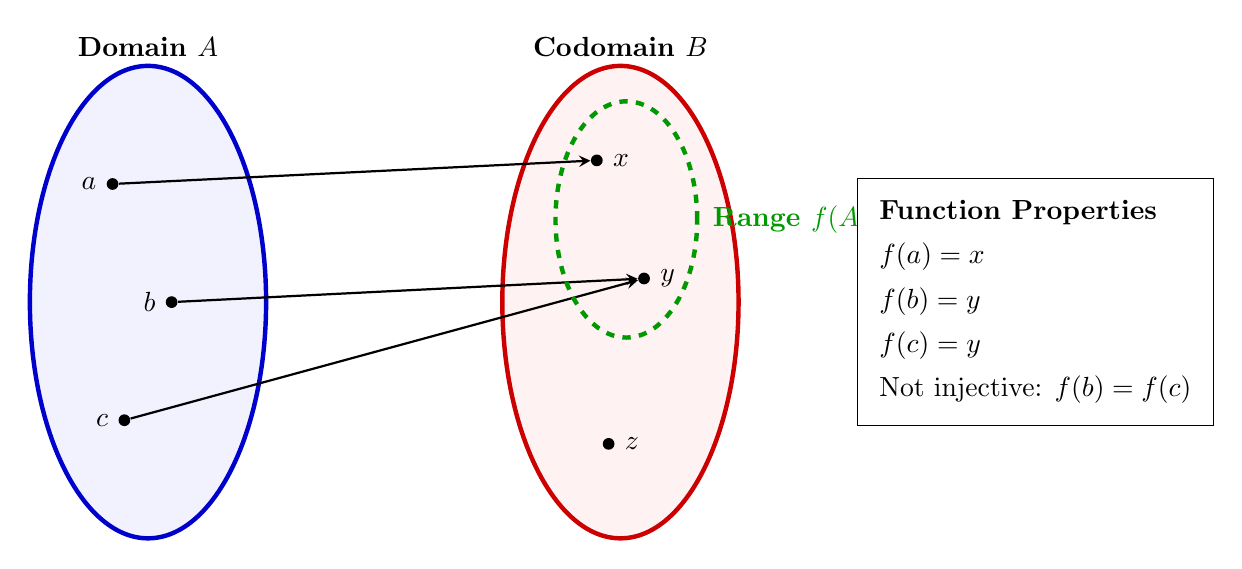
\begin{tikzpicture}[scale=1.5]
    % Backgrounds
    \fill[blue!5] (0,0) ellipse (1 and 2);
    \fill[red!5] (4,0) ellipse (1 and 2);
    
    % Outlines
    \draw[ultra thick, blue!80!black] (0,0) ellipse (1 and 2);
    \draw[ultra thick, red!80!black] (4,0) ellipse (1 and 2);
    
    % Nodes in A
    \node[circle, fill=black, inner sep=1.5pt, label=left:{$a$}] (a) at (-0.3, 1) {};
    \node[circle, fill=black, inner sep=1.5pt, label=left:{$b$}] (b) at (0.2, 0) {};
    \node[circle, fill=black, inner sep=1.5pt, label=left:{$c$}] (c) at (-0.2, -1) {};
    
    % Nodes in B
    \node[circle, fill=black, inner sep=1.5pt, label=right:{$x$}] (x) at (3.8, 1.2) {};
    \node[circle, fill=black, inner sep=1.5pt, label=right:{$y$}] (y) at (4.2, 0.2) {};
    \node[circle, fill=black, inner sep=1.5pt, label=right:{$z$}] (z) at (3.9, -1.2) {};
    
    % Arrows
    \draw[->, >=stealth, thick] (a) -- (x);
    \draw[->, >=stealth, thick] (b) -- (y);
    \draw[->, >=stealth, thick] (c) -- (y);
    
    % Labels
    \node[above, font=\bfseries, text=black] at (0, 2) {Domain $A$};
    \node[above, font=\bfseries, text=black] at (4, 2) {Codomain $B$};
    
    % Range subset
    \draw[dashed, ultra thick, green!60!black] (4.05, 0.7) ellipse (0.6 and 1);
    \node[right, green!60!black, font=\bfseries] at (4.7, 0.7) {Range $f(A)$};
    
    % Legend
    \node[align=left, draw, fill=white, inner sep=8pt, anchor=west, text=black] at (6, 0) {
        \textbf{Function Properties} \\[4pt]
        $\displaystyle f(a) = x$ \\[4pt]
        $\displaystyle f(b) = y$ \\[4pt]
        $\displaystyle f(c) = y$ \\[4pt]
        Not injective: $f(b) = f(c)$
    };
\end{tikzpicture}
\end{center}

\subsection{Heuristics \& Pitfalls}
\begin{itemize}
    \item \textbf{Pitfall - Confusing Image and Preimage Properties:} Remember that the preimage behaves perfectly with all set operations ($f^{-1}(A \cup B) = f^{-1}(A) \cup f^{-1}(B)$ and $f^{-1}(A \cap B) = f^{-1}(A) \cap f^{-1}(B)$). The forward image does \textit{not} behave perfectly with intersections; $f(A \cap B) \subseteq f(A) \cap f(B)$ is the best you can guarantee unless the function is injective.
    \item \textbf{Heuristic - The Horizontal Line Test in Abstract Sets:} To check if a relation is a function, ensure no element in the domain has two arrows leaving it. To check if it is injective, ensure no element in the codomain has two arrows entering it.
\end{itemize}

\newpage
\section{Part 5: Conceptual Synthesis and The "Big Picture"}

\subsection{A) Thematic Connections}
The central theme of this chapter is \textbf{formalizing mappings}. In elementary mathematics, functions are viewed merely as computational formulas. By redefining functions as strict subsets of Cartesian products, we strip away the need for algebraic formulas. This allows us to map abstract entities—such as mapping a set of matrices to a set of polynomials, or mapping a sample space of coin flips to real numbers. This rigorous set-theoretic foundation unifies logic, relations, and algebra into a single cohesive framework.

\subsection{B) Forward and Backward Links}
\textbf{Backward Links:} This topic directly extends the study of relations and Cartesian products. A function is simply a highly disciplined relation. 
\textbf{Forward Links:} Understanding functions at this abstract level is the absolute bedrock for advanced mathematics. In Abstract Algebra, functions that preserve structure are called \textit{homomorphisms}. In Topology, functions that preserve proximity are \textit{continuous maps}. In Measure Theory and Probability, functions that preserve measurable sets are \textit{random variables}. Without the rigorous definition of preimages ($f^{-1}$), modern probability theory (Kolmogorov's axioms) could not exist.

\section{Part 6: Abstract Real-World Modeling (AI, ML, \& Quant Finance)}

\subsection{A) Concrete Scenarios}
\begin{enumerate}
    \item \textbf{Quantitative Finance (Derivative Pricing):} In Stochastic Calculus, the payoff of a financial derivative is modeled as a function mapping a state space of market trajectories to a real-valued payoff. The rigorous definition of preimages is required to ensure this function is "measurable" with respect to the market information available at time $T$.
    \item \textbf{Machine Learning (Loss Functions):} In deep learning, a neural network is a composition of abstract functions $f_{\theta}: \R^n \to \R^m$. The loss landscape is a function mapping the high-dimensional parameter space to a single real number representing the error.
\end{enumerate}

\subsection{B) Model Problem Setup: Measurable Functions in Quant Finance}
Let us build a rigorous mathematical model for pricing a European Call Option. 
Let $(\Omega, \F, \Prob)$ be a probability space, where $\Omega$ is the sample space of all possible continuous stock price trajectories over time $[0, T]$, $\F$ is the $\sigma$-algebra representing the flow of information, and $\Prob$ is the historical probability measure.

A stock price at maturity $T$ is a \textbf{random variable}, which is rigorously defined as a measurable function $S_T: \Omega \to \R$. The condition of measurability requires that for any Borel set $B \subseteq \R$, the preimage satisfies:
\[ S_T^{-1}(B) = \{\omega \in \Omega : S_T(\omega) \in B\} \in \F \]
The payoff of a European call option with strike $K$ is a function $C: \Omega \to \R$ defined by the composition:
\[ C(\omega) = \max(S_T(\omega) - K, 0) \]
Because $S_T$ is a measurable function and the $\max$ function is continuous, their composition $C$ is also a measurable function. The fundamental theorem of asset pricing states that the fair price $V_0$ of this option is the expected value of this function under a risk-neutral measure $\mathbb{Q}$:
\[ V_0 = e^{-rT} \E^{\mathbb{Q}}[C] = e^{-rT} \int_{\Omega} \max(S_T(\omega) - K, 0) \, d\mathbb{Q}(\omega) \]
This demonstrates how the abstract set-theoretic definition of a function and its preimages forms the mathematical architecture required to price billions of dollars in financial derivatives.

\newpage
\section{Part 7: Common Variations and Untested Concepts}

\subsection{Bijective Functions and Invertibility}
While the homework touches on the definition of functions and one-to-one (injective) properties, it omits the formal proof of \textbf{bijectivity} and the existence of an inverse function $f^{-1}: B \to A$ (not to be confused with the preimage of a set). A function is bijective if it is both injective (one-to-one) and surjective (onto).

\textbf{Example Proof:} Prove that the function $f: \R \to \R$ defined by $f(x) = 2x + 3$ is bijective.

\textbf{Proof of Injectivity:} 
Let $x, y \in \R$ and assume $f(x) = f(y)$.
\[ 2x + 3 = 2y + 3 \implies 2x = 2y \implies x = y \]
Since $f(x) = f(y)$ implies $x = y$, the function $f$ is injective.

\textbf{Proof of Surjectivity:}
Let $y \in \R$ be an arbitrary element in the codomain. We must find an $x \in \R$ in the domain such that $f(x) = y$.
Set $2x + 3 = y$ and solve for $x$:
\[ 2x = y - 3 \implies x = \frac{y - 3}{2} \]
Since $y \in \R$, the value $x = \frac{y - 3}{2}$ is also a real number, so $x \in \R$. Furthermore:
\[ f(x) = 2\left(\frac{y - 3}{2}\right) + 3 = (y - 3) + 3 = y \]
Thus, $f$ is surjective. Since $f$ is both injective and surjective, it is bijective. $\blacksquare$

\section{Part 8: Advanced Diagnostic Testing: "Find the Flaw"}

Below are five advanced proofs containing a single, subtle logical flaw. Your task as the grader is to identify the error.

\textbf{Problem 1:} Prove that $f: \R \to \R$ defined by $f(x) = x^2$ is surjective.
\textit{Flawed Proof:} Let $y \in \R$. We need to find an $x \in \R$ such that $f(x) = y$. Let $x = \sqrt{y}$. Then $f(x) = (\sqrt{y})^2 = y$. Since we found such an $x$ for any $y$, $f$ is surjective.

\textbf{Problem 2:} Let $f: A \to B$ be a function. Prove that $f(f^{-1}(E)) = E$ for all $E \subseteq B$.
\textit{Flawed Proof:} Let $y \in E$. By definition of the preimage, there exists $x \in f^{-1}(E)$ such that $f(x) = y$. Therefore, $y \in f(f^{-1}(E))$. This shows $E \subseteq f(f^{-1}(E))$. The reverse inclusion $f(f^{-1}(E)) \subseteq E$ is trivial. Thus $f(f^{-1}(E)) = E$.

\textbf{Problem 3:} Find the domain of $f(x) = \ln(x^2 - 4)$ over the real numbers.
\textit{Flawed Solution:} The argument of the natural logarithm must be strictly positive. We require $x^2 - 4 > 0$. Taking the square root of both sides gives $x > \sqrt{4}$, so $x > 2$. The domain is $(2, \infty)$.

\textbf{Problem 4:} Let $A = \{1, 2\}$ and $B = \{a, b, c\}$. Find the number of injective functions from $B$ to $A$.
\textit{Flawed Solution:} The total number of functions from $B$ to $A$ is $|A|^{|B|} = 2^3 = 8$. Since $|B| > |A|$, not all functions can be injective. We subtract the functions that map all elements to $a$ or all to $b$ (which is 2). So there are $8 - 2 = 6$ injective functions.

\textbf{Problem 5:} Prove that if $f: A \to B$ and $g: B \to C$ are functions, and the composition $g \circ f$ is injective, then $g$ is injective.
\textit{Flawed Proof:} Assume $g \circ f$ is injective. Let $y_1, y_2 \in B$ such that $g(y_1) = g(y_2)$. Since $f$ is a function from $A$ to $B$, there exist $x_1, x_2 \in A$ such that $f(x_1) = y_1$ and $f(x_2) = y_2$. Then $g(f(x_1)) = g(f(x_2))$, which means $(g \circ f)(x_1) = (g \circ f)(x_2)$. Since $g \circ f$ is injective, $x_1 = x_2$. Therefore, $y_1 = f(x_1) = f(x_2) = y_2$. This proves $g$ is injective.

\vspace{1em}
\hrule
\vspace{1em}
\textbf{Solution Key (The Flaws):}
\begin{enumerate}
    \item \textbf{Flaw 1:} The expression $\sqrt{y}$ is not defined in the real numbers for $y < 0$. Because the codomain is $\R$, choosing $y = -1$ yields no real $x$. The function is not surjective.
    \item \textbf{Flaw 2:} The assumption that "there exists $x \in f^{-1}(E)$ such that $f(x) = y$" is false if $y$ is not in the range of $f$. If $y \in E$ but $y \notin \text{range}(f)$, then $f^{-1}(\{y\}) = \emptyset$. The theorem is only true if $f$ is surjective.
    \item \textbf{Flaw 3:} Taking the square root of an inequality $x^2 > 4$ yields $|x| > 2$, not $x > 2$. This means $x > 2$ or $x < -2$. The correct domain is $(-\infty, -2) \cup (2, \infty)$.
    \item \textbf{Flaw 4:} By the Pigeonhole Principle, since the domain $B$ has 3 elements and the codomain $A$ has only 2 elements, it is impossible to map each element of $B$ to a unique element in $A$. There are exactly $0$ injective functions.
    \item \textbf{Flaw 5:} The proof falsely assumes that for any $y_1, y_2 \in B$, there exist preimages $x_1, x_2 \in A$. This assumes $f$ is surjective, which is not given. The correct theorem is that if $g \circ f$ is injective, then $f$ (the inner function) must be injective, not $g$.
\end{enumerate}

\end{document}